\chapter{Introduction to Drawing}

\section{Defining Geometry}

OpenGL can in principle only draw 3 kinds of shapes, known as ``primitives''; triangles, lines and points.

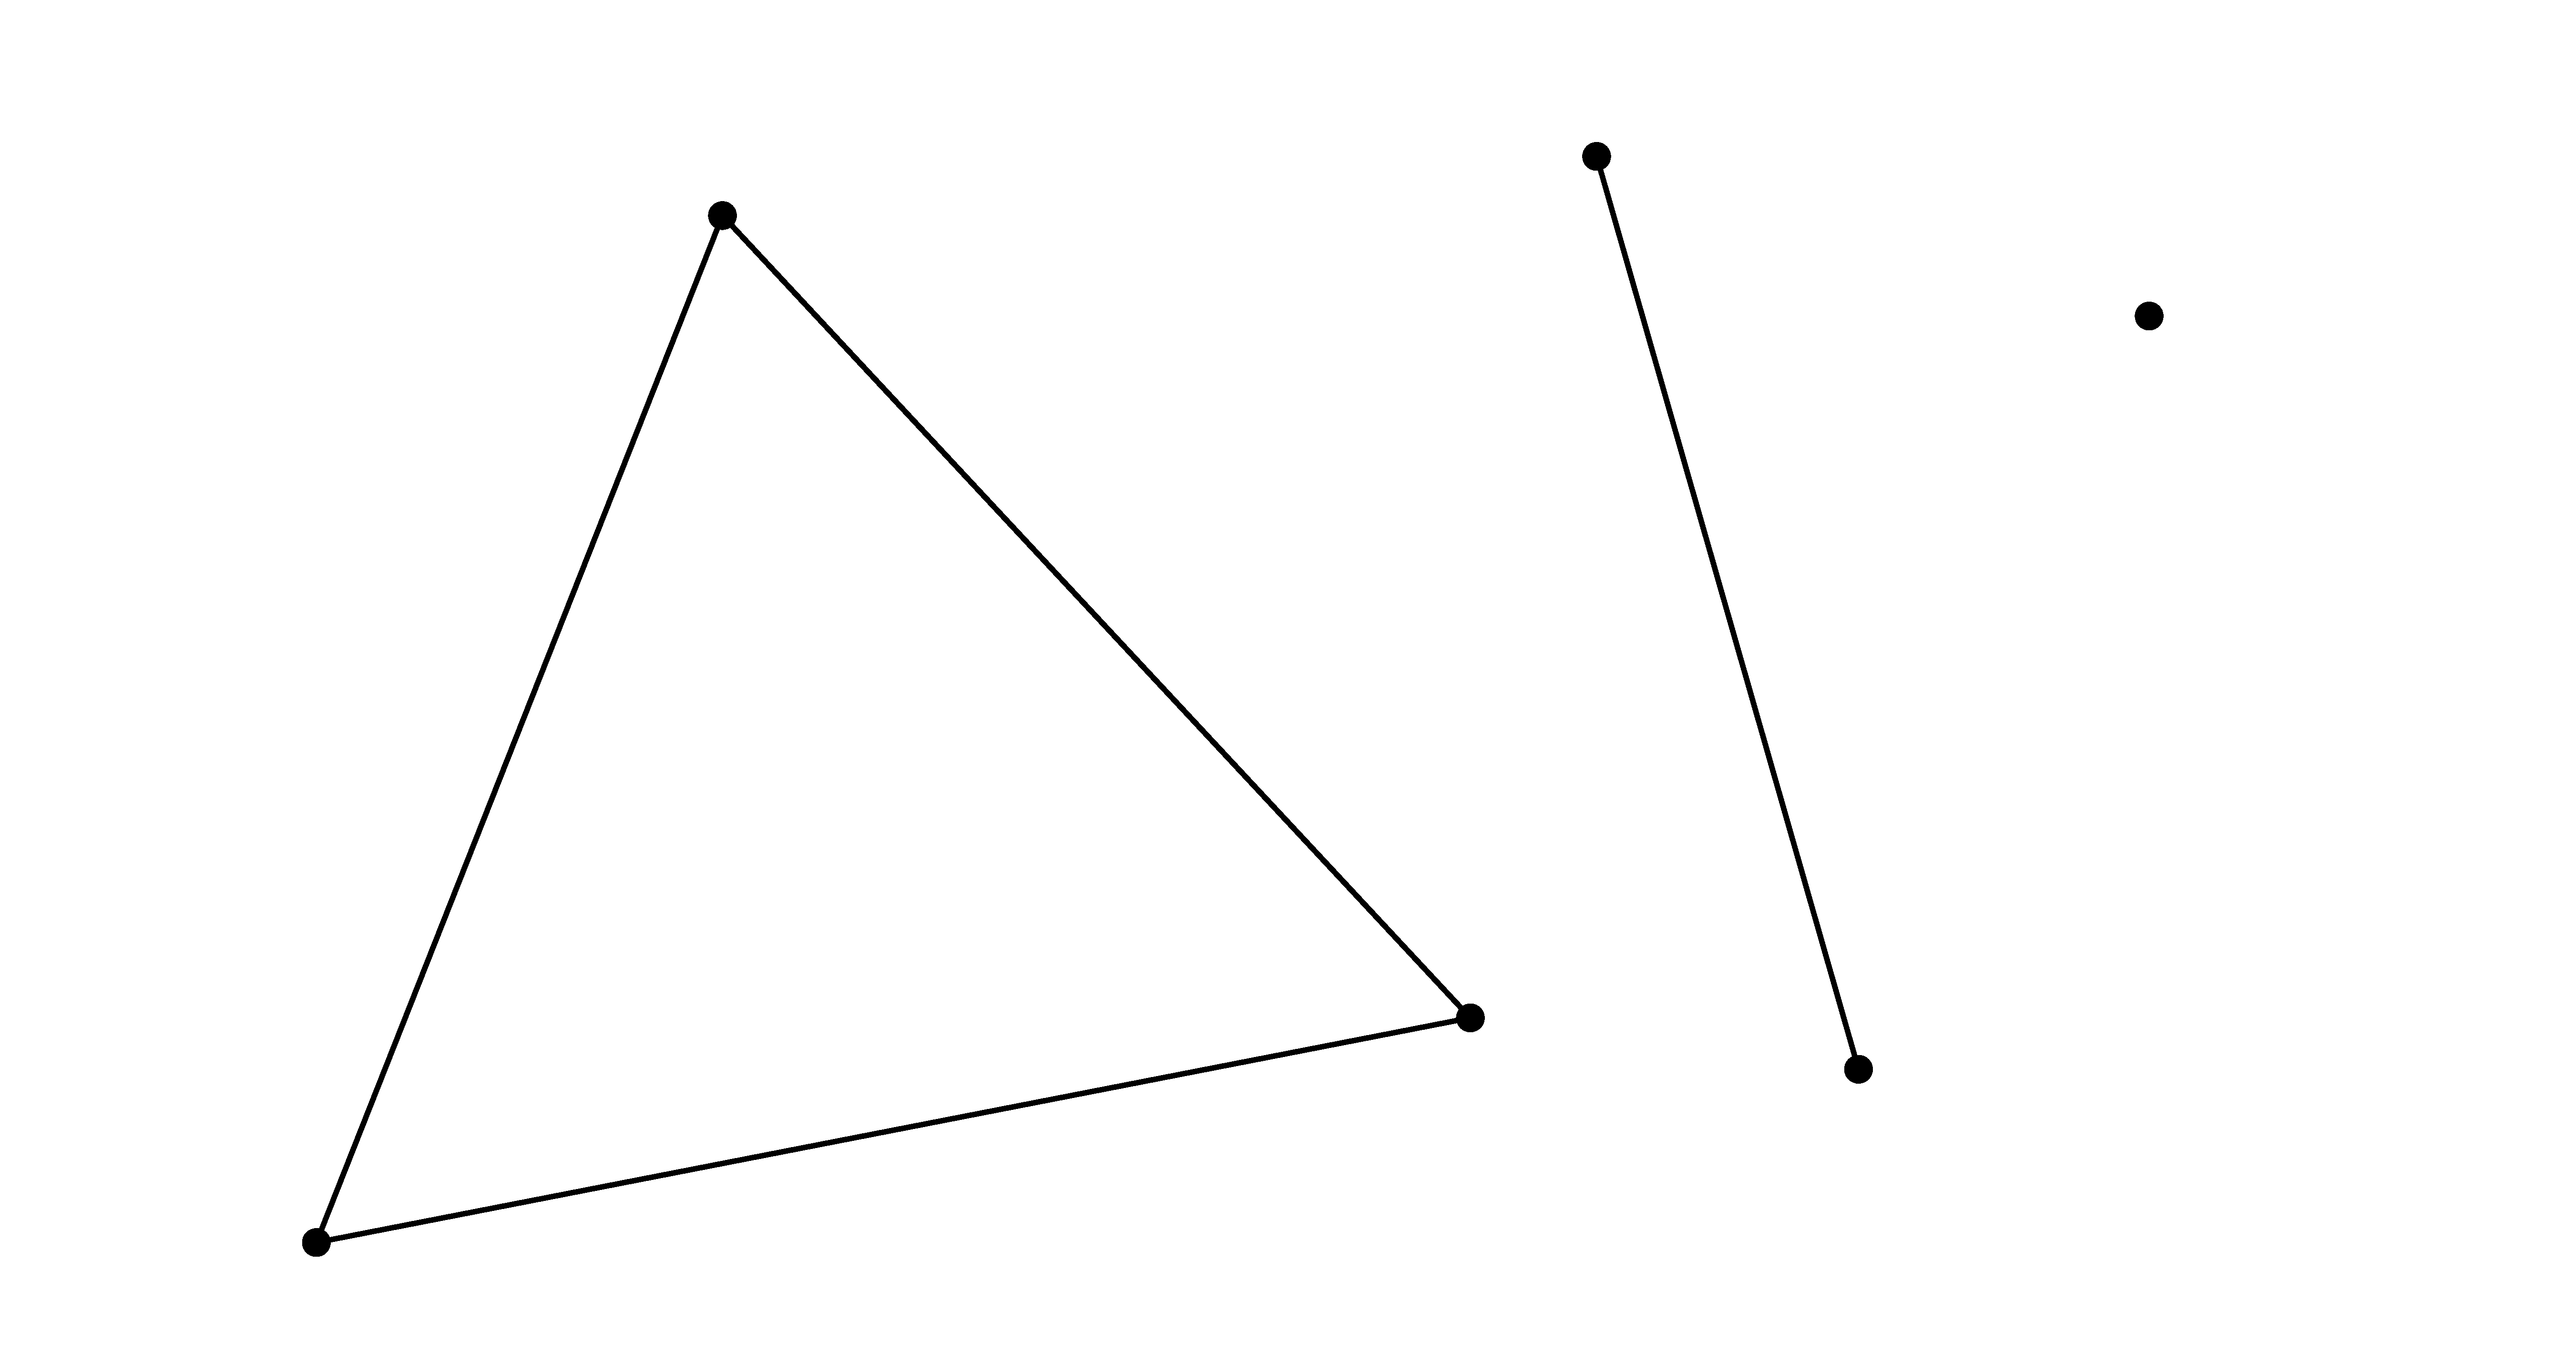
\includegraphics[scale=0.15]{images/openGL_primitives.eps}

Of these three, the triangle is the one that's most commonly used in practice. Primitives combined into shapes are commonly referred to as \emph{geometry}.

Why only three basic shapes? What about rectangles, circles, ellipses, spheres, and so on? 

There are two reasons for this. First, as you will see in the lectures rasterising and rendering triangles is very easy and can therefore be performed very cheaply on the graphics card and accelerated in hardware. Second, you can approximate all the shapes I listed using triangles anyway. 

As mentioned previously, defining a shape in OpenGL consists of defining a list of vertices, which are subsequently combined into primitives that can be rendered. We will now take a look at how these vertex lists can be created, filled with geometry, and prepared to be inserted into the rendering pipeline.

\subsection{Specifying vertices}

The central component in defining a renderable model is an object known as a \emph{Vertex Array Object} (VAO). Its main purpose is linking the contents of input buffers to vertex shader inputs.

\begin{center}
\includegraphics{images/vao-overview.eps}
\end{center}

The illustration above should give a general idea on what is going on. On the left hand side, there are input buffers containing geometry which you'd like to draw. On the right hand side are shown some inputs to the vertex shader, which are defined in the shader source code (don't worry about understanding these variables; we'll deal with them in detail later). 

The link which a VAO represents is the one between data contained inside an input buffer, and an input to the vertex shader. You are responsible for creating these links, and it's easiest to do so while creating the input buffers.

It's common to use a separate VAO for every model in your scene. What the word model \emph{means} in this context depends on what you define it to be. For instance, if you want to render a car, the car's body could be stored in one VAO and the tires in a separate one. It's also possible to store the entire model in a single VAO.

The input buffers used to store input data are known as \emph{Vertex Buffer Objects} (VBO's). The contents of a VBO are generally stored on the memory bank (VRAM) of your graphics card. You therefore have to explicitly transfer data to it before you can use it to draw things.

The sole purpose of VBO's is to hold data. They do not know how their contents are formatted, what their contents represent, nor where their contents are supposed to be used. All of that information is held by the Vertex Array Object.

We'll now look at how you can create your very own Vertex Array Object, followed by how to define and fill a Vertex Buffer Object, and set both up for rendering.

\subsubsection{Creating and setting up a Vertex Array Object}

The first step is to create a new Vertex Array Object using:

\begin{minted}{c}
void glGenVertexArrays(int count, unsigned int* arrayIDs);
\end{minted}

The arrayIDs parameter requires a pointer to a location where the generated array ID(s) can be stored. You are responsible for allocating enough space for these. If not you can cause data corruption or even crashes. For instance, trying to allocate 5 VAO's while passing in an integer array containing 3 entries may cause data corruption on your program stack.

However, the function is relatively easy to use when only allocating a single VAO. Simply create an empty unsigned int on the previous line (\mintinline{cpp}{unsigned int array = 0;}), and pass a reference to it into the function using the \& operator (\mintinline{c}{&array}). The ID of the VAO will be stored in \mintinline{c}{array} afterwards. For simplicity I recommend only generating one VAO at a time unless you really know what you're doing.

The first thing to note here is that you don't actually get a Vertex Array \emph{Object}, but instead the \emph{ID} of the generated VAO. As such you don't actually get to modify the object directly. Instead you use the ID to refer to the array whenever you want to do anything with it. You modify it through OpenGL function calls. 

This is common to the design of all data structures in OpenGL: you only get references instead of complete data structures.

If we want to link Vertex Buffer Objects to shader inputs using the Vertex Array Object, we have to ensure any configuration values are set \emph{while the VAO is active}. You can imagine this process to be like opening a file; in order to add some lines of text (the VBO's) to a text file (the VAO), you first have to open it. As OpenGL is a state machine, this ``file'' will remain open until another one is opened in its place. This process is referred to as \emph{binding}.

Like object references, the concept of binding objects is also used in many other places throughout the OpenGL API. 

The function for binding a vertex array object is defined as follows:

\begin{minted}{c}
void glBindVertexArray(unsigned int vertexArrayID);
\end{minted}

\subsubsection{Creating buffers}

Now that we have created and bound a VAO, we can proceed with defining a Vertex Buffer Object to hold the geometry data of our model. In order to set up a VBO, fill it with data, and create a connection to a shader input in the VAO, there is a particular sequence of functions you need to call. We'll be taking a look at these functions below.

The first step is to create the Vertex Buffer Object. This function works identically to the one used for creating VAO's:

\begin{minted}{c}
void glGenBuffers(int count, unsigned int* bufferIDs);
\end{minted}

Note that even though the buffer is meant to hold data, you don't need to specify the size of your buffer at this point. OpenGL will perform these allocations behind the scenes as you fill or append data to your buffer.

\subsubsection{Binding buffers}

Like Vertex Array Objects, Vertex Buffer Objects are also required to be \emph{bound} before they can be modified, and only one can be bound at a time. 

The function for binding a buffer is:

\begin{minted}{c}
void glBindBuffer(enum target, unsigned int bufferID);
\end{minted}

The target parameter specifies which kind of buffer you would like to bind your buffer as. Most of these types are advanced uses that are not relevant for this course. You'll therefore usually want to pass in \mintinline{c}{GL_ARRAY_BUFFER} here.

The bufferID parameter is the ID of the buffer you would like to work with. This should be the buffer ID you generated using \mintinline{c}{glGenBuffers()}.

It is possible to ``unbind'' a VBO by binding a buffer with an ID of 0. However, it is not something that ought to be done in practice for two reasons. First, any subsequent time a buffer is going to be modified, it will have to be bound first anyway. Second, binding and unbinding buffers may incur additional overhead on the OpenGL driver implementation side.

\subsubsection{Filling buffers}

Now that we have created and bound our buffer, we can fill it with data. This of course requires that you already have some geometry data to fill it with. A general method for doing so is to allocate an array of floats (although other data types will work too):
\begin{minted}{c}
                //   x    y    z    x    y    z    x    y    z  .. and so on
float vertices[] = {1.0, 3.0, 2.0, 5.0, 4.0, 3.0, 2.0, 6.0, 3.0};
\end{minted}

In practice, this data usually originates from a separate file. 

Once you have your float array ready to go, you can use the \mintinline{c}{glBufferData()} function to transfer the data to the GPU:

\begin{minted}{c}
void glBufferData(enum target, size_t size, void* data, enum usage);
\end{minted}

The target parameter has to match the target parameter you supplied in the \mintinline{c}{glBindBuffer()} call.

The size parameter is the size of your data array in bytes. You'll probably need to use the \mintinline{c}{sizeof(/* data type */)} function here, which returns the number of bytes a particular datatype occupies in memory. Note that \mintinline{c}{sizeof()} takes in a datatype as its parameter, such as \mintinline{c}{float} or \mintinline{c}{int}. 

It is in some cases possible to pass the array into the \mintinline{c}{sizeof()} function directly to get the number of bytes occupied by the array's contents in memory.

For instance:

\begin{minted}{c}
int someArray[] = {1, 2, 3};
printf("The size of someArray in bytes is \%i.\n", sizeof(someArray));
// Prints: "The size of someArray in bytes is 12."
\end{minted}

However, whenever an array is passed as a parameter into another function, it is quietly converted into a pointer. This even happens when the function parameter has the array type. As a pointer only represents a memory address, the array dimensions information is lost. As such calling sizeof() on the array variable will give you the size of the pointer (usually 8 bytes on a 64 bit system), rather than the total size of the array.

It may therefore be beneficial to pass in the length of the array into the function as a separate parameter, so this confusing behaviour can be avoided altogether. In that case, multiply the length of the array with the size of the datatype of that array (e.g. \mintinline{c}{arrayLength * sizeof(float)}) to get the size of the array in bytes.

Next is the data parameter, which (surprise surprise) contains a pointer to the data which should be copied to the GPU. Note that the type of this parameter is a \mintinline{c}{void} pointer. A \mintinline{c}{void} pointer in C means that you can supply a pointer to any data type you want. So for instance \mintinline{c}{float*} or \mintinline{c}{int*} are both valid parameter types here.

The usage parameter provides a hint to the purpose of the data you're supplying. Based on this parameter, the OpenGL implementation may perform optimisations to a greater or lesser degree, if at all. It does not restrict how you can use the buffer. 

For basic rendering of models it's best to use \mintinline{c}{GL_STATIC_DRAW} here. The \mintinline{c}{STATIC} component indicates that the contents of the buffer are not expected to change often, if at all. The alternatives for \mintinline{c}{STATIC} are \mintinline{c}{DYNAMIC} and \mintinline{c}{STREAM}, which are intended for increasing modification rates to the buffer.

The \mintinline{c}{DRAW} component indicates that the contents of the buffer are intended for rendering geometry. The alternatives are more advanced uses outside the scope of this guide.

\subsubsection{Format Specification}

You may have noticed from the \mintinline{c}{glBufferData()} function specification that there was no requirement for defining the format of your buffer. OpenGL does not know whether you passed in floats or integers, nor does it know whether you specified x, y and z coordinates, or only x and y coordinates.

For this reason we have to set a \emph{Vertex Attribute Pointer}. A Vertex Attribute is a term used to refer to an input of the vertex shader. A Vertex Attribute Pointer specifies where the vertex shader can obtain the data for a particular vertex attribute and how it is formatted.

Here's the function for setting the Vertex Attribute Pointer:

\begin{minted}{c}
void glVertexAttribPointer(
    unsigned int index, 
    int size, 
    enum type, 
    bool normalised, 
    size_t stride, 
    void* pointer
);
\end{minted}

Even more parameters than \mintinline{c}{glBufferData()}! Let's go over them.

The index parameter specifies the index of the vertex attribute pointer you would like to set. Don't worry if that doesn't make sense right now, we'll come back to it in the section about Shaders. In a nutshell you give each Vertex Attribute in the vertex shader a number, and use the same number in this function to connect the VBO to the Vertex Attribute.

This is a number you can make up yourself, as long as it is between 0 and the OpenGL constant \mintinline{c}{GL_MAX_VERTEX_ATTRIBS}, and you use the same IDs for the same Vertex Attribute both in OpenGL function calls as well as your Shader source code. 

Note that the values of OpenGL constants need to be queried. You can find out the value of the constant by using:

\begin{minted}{c}
int maxVertexAttribs;
glGetIntegerv(GL_MAX_VERTEX_ATTRIBS, &maxVertexAttribs);
printf("GL_MAX_VERTEX_ATTRIBS: %i\n", maxVertexAttribs);
\end{minted}

On modern machines, this value is almost always 16.

The size parameter can either be 1, 2, 3 or 4. It defines the number of components per \emph{entry} in the buffer. For instance, only specifying x and y coordinates per vertex means that \mintinline{c}{size} should be 2. If you specify x, y and z coordinates, \mintinline{c}{size} is 3, and so on.

\mintinline{c}{Type} defines the data type of the values in the buffer. This should match the type of values you passed in with the \mintinline{c}{glBufferData()} call. Here's some of the possible data types you can pass in here:

\begin{itemize}
	\item \mintinline{c}{GL_BYTE}
	\item \mintinline{c}{GL_UNSIGNED_BYTE}
	\item \mintinline{c}{GL_SHORT}
	\item \mintinline{c}{GL_UNSIGNED_SHORT}
	\item \mintinline{c}{GL_INT}
	\item \mintinline{c}{GL_UNSIGNED_INT}
	\item \mintinline{c}{GL_FLOAT}
\end{itemize}

Performance tip: you should always choose the smallest possible data type possible that is acceptable for your data. For instance, if you have a buffer of positive integers whose values never exceed 255, you can make indices of the type \mintinline{c}{GL_UNSIGNED_BYTE}. Doing this can significantly reduce the memory bandwidth requirements of the graphics card, increasing performance.

Next up is the \mintinline{c}{normalised} parameter. It defines whether OpenGL should normalise the values in your buffer. In most cases you'll want to pass \mintinline{c}{GL_FALSE} here. 

The \mintinline{c}{stride} parameter defines the number of bytes between each \emph{entry} in the buffer. This may sound strange at first; if a buffer only contains coordinates, can't you just calculate these from the other parameters? The thing is that if you want, a single Vertex Buffer Object can contain multiple Vertex Attributes. For instance, you can pack both vertex coordinates and texture coordinates \footnote{In a nutshell, textures are images that can be mapped on to triangles. Texture Coordinates tell OpenGL what part of such an image to project on a given triangle. Since textures are (usually) two-dimensional objects, you can use two coordinates to define locations on the texture itself. The ``u'' and ``v'' names by which each axis is often referred to is the origin of the other common name for textures; UV maps.} in the same buffer:

\centerline{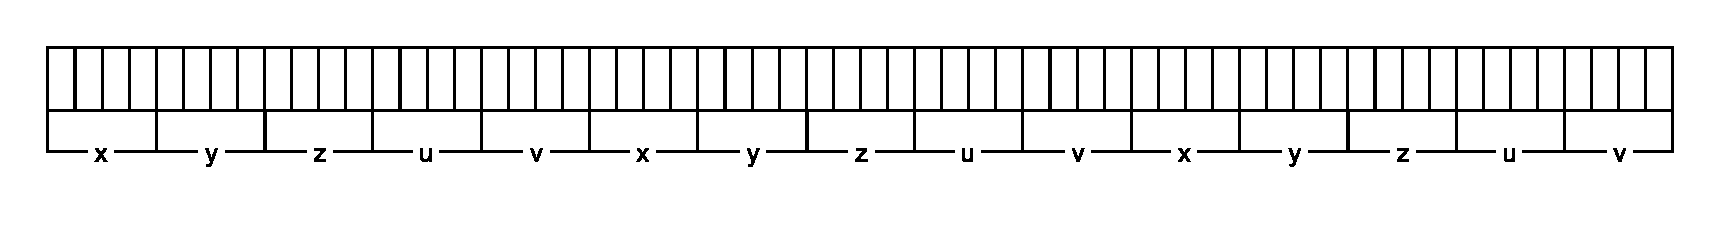
\includegraphics[scale=0.6]{images/openGL_interleaved_buffer.eps}}

In this case, the buffer contains 3 floating point coordinate components (x, y, and z) of 4 bytes each, as well as 2 texture coordinates of 4 bytes each. The number of bytes from the first byte of an x coordinate to the next is 20 bytes. This is known as the \emph{stride}. 

If your buffer only contains a single entry type, you can pass in 0 here, and OpenGL will deduce the stride for you based upon the values of other parameters. However, when multiple entry types are present such as in the example shown above, you're responsible for determining the proper stride yourself.

Finally, the \mintinline{c}{pointer} parameter defines the number of bytes until the first value in the buffer. Using the example from the buffer shown above, the x, y and z coordinates start at index 0, while the texture coordinates start at byte $3 \cdot 4 = 12$. If you only have a single entry type in your buffer, this parameter is usually 0.

\subsubsection{Enabling the Vertex Attributes}

Finally, we need to enable the Vertex Buffer Objects that should serve as input to the rendering pipeline. Inputs can be enabled with: 

\begin{minted}{c}
void glEnableVertexAttribArray(unsigned int index);
\end{minted}

The index parameter should correspond to the index you passed into the \mintinline{c}{glVertexAttribPointer()} while setting up the VAO. You need to call \mintinline{c}{glEnableVertexAttribArray()} once for every Vertex Attribute you would like to use as input for rendering.

Calling \mintinline{c}{glVertexAttribPointer()} and \mintinline{c}{glEnableVertexAttribArray()} ensures the Vertex Attributes are linked to shader inputs when you issue a draw call. 

And that's it! Your Vertex Attribute is now active within the VAO, ready to be used. However, there's one more step before we can draw its contents.

\subsection{The index buffer}

We now have a buffer which defines the coordinates of a number of vertices. However, we did not specify any information about how these are supposed to be combined into primitives. We can do this through the use of a special buffer called an ``index buffer''. 

You might wonder why we have to specify an additional buffer to combine vertices into primitives instead of just using the vertices in the order they are defined in your VBO? To answer this, let's take a look at a cube made up of triangles:\\

\centerline{\includegraphics[scale=0.3]{images/cube.png}}

Notice how most vertices are part of multiple triangles. The center one is even part of 4 of them. 3D surfaces tend to be ``watertight'' in order to appear convincing on the rendered image. As this requires using the same vertices several times over for different triangles, it makes sense to only define the vertices once, and combine them together by referring to their \emph{index} in the VBO. If executed well, you can save quite a bit of memory usage. 

This process is comparable to the ``connect the dots'' puzzles, where a set of vertices with associated indices are defined which can be connected into a shape. The only difference here is that vertices with arbitrary indices can be combined into points, lines, triangles or otherwise. An example of such a puzzle is shown below \footnote{Original image by whitney waller, red lines added - connect-the-dots, CC BY-SA 2.0, https://commons.wikimedia.org/w/index.php?curid=45762476}:

\centerline{\includegraphics[scale=0.3]{images/Connect_the_dots_puzzle_(partially_solved).png}}

Fortunately, the mechanism for creating and filling an index buffer is very similar to the way we set up VBO's. I'll therefore only outline the differences here.

First, you generate another buffer using \mintinline{c}{glGenBuffers()}.

Next, you bind the generated buffer with as target \mintinline{c}{GL_ELEMENT_ARRAY_BUFFER}, as opposed to \mintinline{c}{GL_ARRAY_BUFFER}. The index buffer has a special ``status'' within the Vertex Array Object and thus has a separate buffer type.

Now we can fill the buffer with indices. They should be unsigned integers, unsigned shorts or unsigned chars (bytes). Just like with the VBO's you should create an array of these. The index of the vertices you defined in your VBO start counting at 0.

Finally, we call \mintinline{c}{glBufferData()} to copy the integer array into the index buffer. Note that the target should in this case also be \mintinline{c}{GL_ELEMENT_ARRAY_BUFFER}.

And we're done! We're now ready to draw our Vertex Array Object :)

Unlike the VBO's, you don't need to call \mintinline{c}{glVertexAttribPointer()} to set up your index buffer.

\newpage
\subsubsection{Visualised Example}

\makebox[\textwidth]{\includegraphics[width=210mm]{images/VAO_initial.pdf}}

Now that we've seen the functions needed to create and fill VBO's and set up a VAO, let's pause for a moment and take a closer look at a practical example to see what effect calling each function in the setup process has.

We'll start with a situation where we've already created some VBO's containing input for the rendering pipeline. We've also created an empty vertex array object. Note that in practice, a VAO really is nothing more than a table containing an entry for each possible vertex attribute index, plus a pointer to an index buffer. This table is created by OpenGL internally, so it's not something you create yourself. 

Finally, there is some shader code on the right hand side of the diagram. We'll come back to shaders in detail in a later chapter, but what's relevant here is that the \mintinline{glsl}{in} keyword declares an input variable to the shader. Additionally, the \mintinline{glsl}{layout(location=0)} qualifier refers to a vertex attribute index, and \mintinline{glsl}{vec3} and \mintinline{glsl}{vec4} are floating point vectors of 3 and 4 elements, respectively. 

\makebox[\textwidth]{\includegraphics[width=210mm]{images/VAO_vert.pdf}}

As mentioned earlier, after having created and filled a VBO, we can use the function \mintinline{c}{glVertexAttribPointer()} to specify the format of our input buffer. 

As indicated, the number of components (or values) per entry in the buffer is 3. Also their datatype (float) is stored in the table.

Note that the buffer contains definitions of vertices as well as vertex surface normal vectors (used in lighting calculations, amongst other things). This affects the stride of the vertex attribute. Since the buffer only contains floating point numbers, each element in the entire buffer uses 4 bytes of space. There are 6 elements from one entry to the next, which means $4 \cdot 6 = 24$ bytes of stride between each entry.

The requirement for having the source VBO bound when calling \mintinline{c}{glVertexAttribPointer()} is due to a pointer being stored to the first byte of the vertex attribute contents. 

\newpage

\makebox[\textwidth]{\includegraphics[width=210mm]{images/VAO_vert_enabled.pdf}}

Remember the need to call the \mintinline{c}{glEnableVertexAttribArray()} function? Here you can see its result. It simply marks a vertex attribute in the vertex array object as enabled, thereby completing the connection from the VAO to a shader input. Since entries are disabled by default, you're responsible to enabling those which you need for rendering.

Notice the effective result thus far: input data which can be located in arbitrary buffers with arbitrary sizes and formatting can be sent as input to arbitrary shaders. 

\newpage

\makebox[\textwidth]{\includegraphics[width=210mm]{images/VAO_norm.pdf}}

The story is fairly similar as for the first vertex attribute. The only difference here is that the input data for the vertex normals start at a later point in the VBO. As you can see, there's a vertex coordinate which precedes it. 

This is a situation where the starting byte of the buffer needs to be adjusted. To do so, you can use the final parameter of the \mintinline{c}{glVertexAttribPointer()}. In this case, there are 3 floats of 4 bytes each preceding the first byte of the vertex normals attribute. This yields a starting byte of 12, which has been indicated separately in the VAO table.

However, the starting byte does not affect the stride, which is the same for both cases.

In the case of vertex normals, which by definition ought to be normalised, it is possible to enable normalisation using a parameter of the \mintinline{c}{glVertexAttribPointer()} function. In this example it has mainly been enabled for the sake of showing a situation where it could be useful, though in practice it's not always a necessity.

\newpage

\makebox[\textwidth]{\includegraphics[width=210mm]{images/VAO_norm_enabled.pdf}}

Again we call \mintinline{c}{glEnableVertexAttribArray()} to create a connection between the VAO entry and the shader input. Note that unlike the VBO's there's no connection created between the VAO and a shader. Instead, think of it as ``opening the floodgates'' to allow input values to flow from the VBO's to a shader input. 

Not calling \mintinline{c}{glEnableVertexAttribArray()} will therefore prevent any inputs from reaching their respective shader input.

\newpage

\makebox[\textwidth]{\includegraphics[width=210mm]{images/VAO_colour.pdf}}

Here's one more attribute for good measure. There are a few things different with this one. First, the data for this vertex attribute originates from a different VBO. Again, this assumes ``buffer\#0'' was bound while calling \mintinline{c}{glVertexAttribPointer()}. 

Second, this buffer object has 4 elements per entry rather than 3. This results in there being 4 entries * 4 bytes per entry = 16 bytes between the start of each subsequent entry, which is the stride. 

\newpage

\makebox[\textwidth]{\includegraphics[width=210mm]{images/VAO_colour_enabled.pdf}}

And finally we enable the attribute using a call to \mintinline{c}{glEnableVertexAttribArray()}. Hopefully you have gotten the idea at this point.

\section{Drawing Vertex Array Objects}

\subsection{Overview}

So where have we gotten up to this point? Here's a diagram showing the buffers we set up:

\centerline{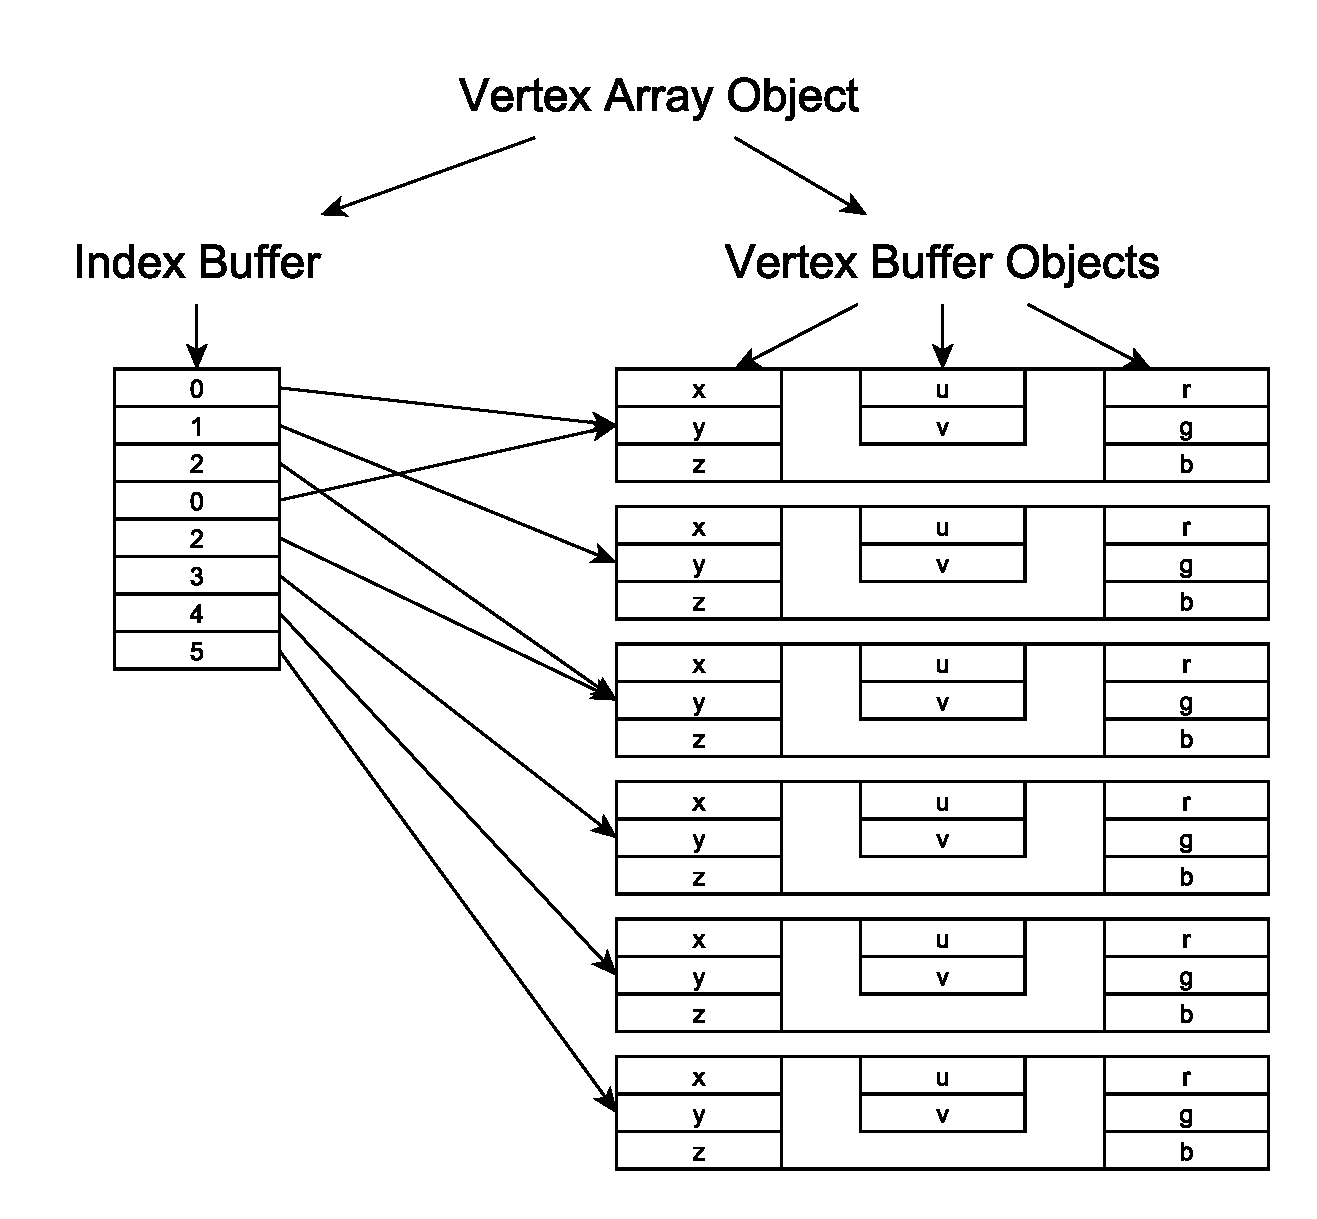
\includegraphics[scale=0.6]{images/openGL_index_buffer.eps}}

We have created a Vertex Array Object which consists of reference to an Index Buffer and references to one or more Vertex Buffer Objects. The Vertex Array Object also contains Vertex Attribute specifications, which a vertex shader can take as input. All a vertex shader needs to do at this point is specify which input should draw its data from which Vertex Attribute.

We will now see how to initiate this rendering process. Don't worry, it's a lot simpler than setting up the VAO!

\subsection{Drawing the Vertex Array Object}

As the frame buffer has to be cleared every frame (the handout code already contains a call to \mintinline{c}{glClear()}), you have to redraw the scene every single frame. Drawing a scene usually happens in a loop known as the ``main loop''. The handout code already has one set up for you. You can insert your drawing calls in there.

The first step of drawing a VAO is to bind it. This works exactly the same way as when we set it up; a single call to \mintinline{c}{glBindVertexArray()}. After this, any drawing command will use this VAO as input. You can only draw from a single VAO at a time.

\subsubsection{Issuing the draw command}

As we have already set up the VAO in its entirety previously, OpenGL already knows how to interpret the various Vertex Buffer Objects, and which Vertex Attributes they will provide. As such we just have to call a single function to draw the VAO:

\begin{minted}{c}
void glDrawElements(enum mode, int count, enum type, void* indices);
\end{minted}

\mintinline{c}{glDrawElements} will cause a draw call to be issued, and use the Vertex Attributes specified in the VAO as input to the rendering pipeline. 

The \mintinline{c}{mode} parameter specifies the type of primitive you'd like to draw. The basic primitive modes are \mintinline{c}{GL_POINTS}, \mintinline{c}{GL_LINES} and \mintinline{c}{GL_TRIANGLES}.

Here are some other handy drawing modes that combine the basic primitives:
\begin{description}
\item[\mintinline{c}{GL_LINE_STRIP}] \hfill \\
		Start with one vertex. For every vertex that follows, draw a line from the previous vertex to the current one.
\item[\mintinline{c}{GL_LINE_LOOP}] \hfill \\
		Same as \mintinline{c}{GL_LINE_STRIP}, but adds an additional line from the last to the first vertex.
\item[\mintinline{c}{GL_TRIANGLE_STRIP}] \hfill \\
		Works similar to a line strip, but uses the previous 2 vertices and the current vertex as coordinates of the triangle. 
\item[\mintinline{c}{GL_TRIANGLE_FAN}] \hfill \\
		Handy for drawing circles. Start with a centre vertex and a vertex on the edge of the circle. Every vertex you add draws a triangle through the centre vertex, the previous and the current one.
\end{description}

The \mintinline{c}{count} parameter specifies how many elements from the index buffer should be drawn. Note that this is the \emph{number of elements}, not the \emph{number of triangles, lines or points}. For example, in the case of \mintinline{c}{GL_TRIANGLES}, \mintinline{c}{count} should always be a multiple of 3.

\mintinline{c}{Type} specifies the data type of the values in your index buffer. This is usually \mintinline{c}{GL_UNSIGNED_INT}, although \mintinline{c}{GL_UNSIGNED_SHORT} and \mintinline{c}{GL_UNSIGNED_BYTE} are also accepted if you happened to specify your indices using those data types.

Finally, \mintinline{c}{indices} specifies the start index in your index buffer to start drawing from. Just pass in 0 here.

Unfortunately, we're not quite ready yet to draw your VAO. As mentioned previously, the rendering pipeline by default is missing a vertex and fragment shader. We'll need to specify those before we can send any draw calls through the pipeline.